\section{Experiment}
\subsection{Settings}
\begin{frame}
  \frametitle{Experiment Settings --- Simulation Settings}
  Sleep-based Simulation
  \begin{itemize}
    \item Sample from obtained data center logs.
    \item Take allocated CPUs as task amount and assign random numbers
      as job priorities.
    \item Sleep according to the execution time.
    \item 20 worker instances used.
    \item Homogeneous/Heterogeneous environments
  \end{itemize}
  \begin{exampleblock}{Penalty Measure}
    \centering
    $\sum Priority * Deadline\, missed$
  \end{exampleblock}
\end{frame}
\begin{frame}
  \frametitle{Experiment Settings --- Comparison Targets}
  \begin{itemize}
    \item Priority-based Policy (similar to JPPF)
    \item Deadline-based Policy with spare resource allocated in order
      of
      \begin{itemize}
        \item Priority
        \item Deadline
      \end{itemize}
    \item Earliest Deadline First Algorithm (an optimal algorithm in
      RTS)
  \end{itemize}
\end{frame}
\begin{frame}
  \frametitle{Experiment Settings --- Hardware}
  \begin{itemize}
    \item Intel Core i5 3570 (2C4T)
    \item 16GB RAM
    \item Ubuntu 14.04 LTS
    \item Ruby 2.1.1
  \end{itemize}
\end{frame}

\subsection{Homogeneous}
\begin{frame}
  \frametitle{Experiment Results --- Homogeneous Environment}
  \begin{itemize}
    \item Tasks in a job have identical sleep time.
    \item Each worker simply sleeps the time hold by that task.
  \end{itemize}
\end{frame}

\begin{frame}
  \frametitle{Experiment Results --- Homogeneous Environment}
  \begin{figure}[htbp]
    \centering
    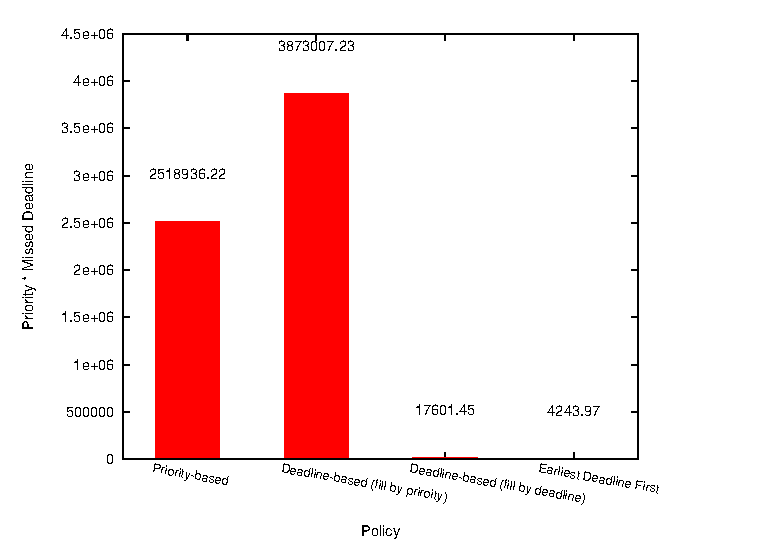
\includegraphics[width=\textwidth,height=0.7\textheight,keepaspectratio]{figures/homo.eps}
    \caption{Homogeneous Environment Setting}
    \label{fig:homo-exp}
  \end{figure}
\end{frame}

\subsection{Heterogeneous}
\begin{frame}
  \frametitle{Experiment Results --- Heterogeneous Environment}
  \begin{itemize}
    \item Specify different worker parameters to represent different
      computing speed.
    \item Sleep time of a task becomes
      \begin{center}
        \begin{minipage}{.8\textwidth}
          \begin{exampleblock}{}
            \centering
            $\left(1 + rand([0-worker\_parameter])\right)*task\_sleep\_time$
          \end{exampleblock}
        \end{minipage}
      \end{center}
    \item Pick 1/20 of the task as GPU task and 4 out of 20 workers as
      GPU server.  When GPU task is send to a GPU worker, its sleep
      time is reduced to 1/10.
  \end{itemize}
\end{frame}

\begin{frame}
  \frametitle{Experiment Results --- Heterogeneous Environment}
  \begin{figure}[htbp]
    \centering
    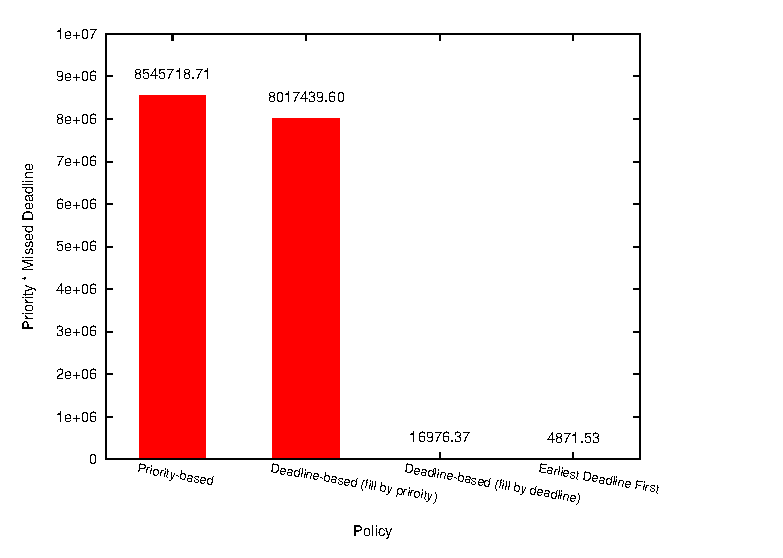
\includegraphics[width=\textwidth,height=0.7\textheight,keepaspectratio]{figures/hetero.eps}
    \caption{Heterogeneous Environment Setting}
    \label{fig:hetero-exp}
  \end{figure}
\end{frame}

